\documentclass[sigplan,10pt]{acmart}

\AtBeginDocument{%
  \providecommand\BibTeX{{%
    \normalfont B\kern-0.5em{\scshape i\kern-0.25em b}\kern-0.8em\TeX}}}

\usepackage{enumerate}
\usepackage{xspace}
\usepackage[labelformat=simple]{subcaption}
\usepackage{tikz}
\usepackage{fancyvrb}
\usepackage{xcolor}
\usepackage{breqn}

% commands
\renewcommand\thesubfigure{(\alph{subfigure})}
\newcommand{\tDelta}{\textsf{Delta}\xspace}

% tikz
\usetikzlibrary{decorations.pathmorphing}
\tikzstyle{vertex} = [circle, minimum width=10pt,draw,inner sep=0pt]
\tikzstyle{vertex2} = [circle, minimum width=40pt,draw,inner sep=0pt]
\tikzstyle{server} = [rectangle, rounded corners,minimum width=2cm,minimum height=2.5cm,draw=black]
\tikzstyle{local} = [thick,->,>=stealth]
\tikzstyle{dist} = [thick,dashed,->,>=stealth]
\tikzstyle{node}=[circle,draw,radius=0.3, align=center]

% colours
\definecolor{grey}{rgb}{0.52, 0.52, 0.51}
\definecolor{red}{rgb}{0.7, 0.11, 0.11}
\definecolor{blue}{rgb}{0.0, 0.0, 0.55}
\definecolor{green}{rgb}{0.0, 0.42, 0.24}

\setcopyright{acmcopyright}
\copyrightyear{2020}
\acmYear{2020}
\acmDOI{10.1145/1122445.1122456}

%% These commands are for a PROCEEDINGS abstract or paper.
\acmConference[PaPoC '20]{PaPoC '20: Proceedings of the 7th Workshop on Principles and Practice of Consistency for Distributed Data}{April 27, 2020}{Heraklion, Crete, Greece}
\acmBooktitle{PaPoC '20: Proceedings of the 7th Workshop on Principles and Practice of Consistency for Distributed Data, April 27, 2020, Heraklion, Crete, Greece}
\acmPrice{15.00}
% \acmISBN{978-1-4503-XXXX-X/18/06}

% Submission ID.
% Use this when submitting an article to a sponsored event. You'll
% receive a unique submission ID from the organizers
% of the event, and this ID should be used as the parameter to this command.
%\acmSubmissionID{123-A56-BU3}

\begin{document}

\title{Preserving Reciprocal Consistency in Distributed Graph Databases}

\author{Jack Waudby}
\email{j.waudby2@ncl.ac.uk}
\affiliation{%
  \institution{Newcastle University}
  \city{Newcastle}
  \country{UK}
  \postcode{NE4 5TG}
}

\author{Paul Ezhilchelvan}
\email{paul.ezhilchelvan@ncl.ac.uk}
\orcid{0000-0002-6190-5685}
\affiliation{%
  \institution{Newcastle University}
  \city{Newcastle}
  \country{UK}
  \postcode{NE4 5TG}
}

\author{Jim Webber}
\email{jim.webber@neo4j.com}
\affiliation{%
  \institution{Neo4j}
  \streetaddress{Union House,182-194 Union Street}
  \city{London}
  \country{UK}
  \postcode{SE1 0LH}}

\author{Isi Mitrani}
\email{isi.mitrani@ncl.ac.uk}
\orcid{0000-0002-7797-7755}
\affiliation{%
  \institution{Newcastle University}
  \city{Newcastle}
  \country{UK}
  \postcode{NE4 5TG}
}

\renewcommand{\shortauthors}{Waudby, et al.}

\begin{abstract}
  Our earlier work identifies \emph{reciprocal consistency} as an important property that must be preserved in distributed graph databases.
  It also demonstrates that a failure to do so seriously undermines the integrity of the database itself in the long term.
  Reciprocal consistency can be maintained as a part of enforcing any known isolation guarantee and such an enforcement is also known to lead to reduction in performance. Therefore, in practice, distributed graph databases are often built atop BASE databases with no isolation guarantees, benefiting from good performance but leaving them susceptible to corruption due to violations of reciprocal consistency.
  This paper designs and presents a lightweight, locking-free protocol and then evaluates the protocol's abilities to preserve reciprocal consistency and also offer good throughput. Our evaluations establish that  the protocol can offer both integrity guarantees and sound performance when the value of its parameter is chosen appropriately.
\end{abstract}

% \begin{CCSXML}
% <ccs2012>
%  <concept>
%   <concept_id>10010520.10010553.10010562</concept_id>
%   <concept_desc>Computer systems organization~Embedded systems</concept_desc>
%   <concept_significance>500</concept_significance>
%  </concept>
%  <concept>
%   <concept_id>10010520.10010575.10010755</concept_id>
%   <concept_desc>Computer systems organization~Redundancy</concept_desc>
%   <concept_significance>300</concept_significance>
%  </concept>
%  <concept>
%   <concept_id>10010520.10010553.10010554</concept_id>
%   <concept_desc>Computer systems organization~Robotics</concept_desc>
%   <concept_significance>100</concept_significance>
%  </concept>
%  <concept>
%   <concept_id>10003033.10003083.10003095</concept_id>
%   <concept_desc>Networks~Network reliability</concept_desc>
%   <concept_significance>100</concept_significance>
%  </concept>
% </ccs2012>
% \end{CCSXML}

\ccsdesc[500]{Data Management~Graph Databases}
\ccsdesc[300]{Data Management~Reciprocal Consistency}
\ccsdesc[300]{Data Management~Concurrency Control}

\keywords{Graph Databases, Reciprocal Consistency, BASE}

\maketitle

\section{Introduction}
\label{sec:introduction}

Recent years have seen a proliferation in the use of graph processing technologies \cite{Besta2019}. Application areas are wide reaching from healthcare, to social networks and fraud detection \cite{Eifrem2016}. Graph databases model data as a \textit{property graph} \cite{Robinson2015}, vertices represent entities and edges represent the relationships between entities. In addition, properties can be stored on both vertices and edges. In the storage layer, edges are represented by two reciprocal pointers, one stored with each vertex the edge connects. This allows for bi-directional traversal and improved query performance \cite{Robinson2015}. An edge is said to be \emph{reciprocally consistent}, if its two end pointers are mutually reciprocal of each other (details in Section \ref{sec:recipr-cons}).

In practice, graphs can be extremely large, sometimes in the magnitude of 100 billion edges \cite{Sahu2017}, exceeding the storage capacity of a single-node graph database and motivating the need for distributed graph databases. A common distributed graph database design pattern is to first partition graph data over several machines in a cluster; resulting in a number of \emph{distributed edges}, an edge's reciprocal pointers reside in different partitions. Recent work \cite{Ezhilchelvan2018} and \cite{Webber2019} highlighted that violations of reciprocal consistency in distributed edges introduce corruption into the database. Moreover, due to the \emph{Scale-Free} \cite{ScaleFree} property exhibited by many real world graphs, this corruption can propagate through the database at alarmingly rates.

When, for example, a BASE database \cite{Pritchett2008} is adapted with a graph processing layer, then violations of reciprocal consistency will occur if that adaptation provides no concurrency control for operations that span partitions in order to offer higher performance. This paper proposes a simple concurrency control protocol, called \tDelta protocol, that does not impede performance adversely. That is because the protocol is exclusively designed for one purpose only: reciprocal consistency in distributed edges.  Its design leverages the fact that the updating of end pointers of a given distributed edge immediately follow each other and the small interval between them is the window for possible conflicts between concurrent updates.

The paper is organized as follows: Section \ref{sec:recipr-cons} presents reciprocal consistency, Sections \ref{sec:distr-graph-datab}-\ref{sec:db-corruption} discuss the architecture of distributed graph databases and describes how corruption occurs. Section \ref{sec:tdelta-protocol} outlines the \tDelta protocol. Sections \ref{sec:modeling}-\ref{sec:evaluation} presents the model used to evaluate protocol performance.


\section{Reciprocal Consistency}
\label{sec:recipr-cons}

In the property graph data model, edges have direction and each edge runs from a \emph{source} vertex to a \emph{destination} vertex.
In the storage layer, however, edge directionality does not exist;  \textbf{both} the source and the destination vertices store information about each other.
This allows edge traversal to be bidirectional and speeds up query performance.

Consider, for example, the statement: ``Tolkien \textit{wrote} The Hobbit''.
It is expressed using vertex  \emph{a} for Tolkien and vertex \emph{b} for The Hobbit, and an edge \textit{wrote} running from \emph{a} (source) to \emph{b} (destination). Corresponding openCypher \cite{openCypher} code is given below and Fig \ref{rc-edge} shows the model level view.% of edge $ab$.
\begin{Verbatim}[commandchars=\\\{\},fontsize=\small,xleftmargin=.2in]
\textcolor{blue}{MATCH} (a:\textcolor{green}{Person}), (b:\textcolor{green}{Book})
\textcolor{blue}{WHERE} a.\textcolor{red}{name} = 'Tolkien' \textcolor{blue}{AND} b.\textcolor{red}{title} = 'The Hobbit'
\textcolor{blue}{CREATE} (a)-[w:\textcolor{green}{WROTE}]->(b)
\end{Verbatim}

Fig \ref{db-rep} depicts the internal representation of a graph arising from JanusGraph \cite{janusgraph} and TitanDB \cite{TitanDB}.
A vertex, such as \emph{a}, is represented by a record that contains one or more properties of that vertex, followed by a sequence of \emph{edge pointers} pointing to all those vertices to which this vertex is related either as a source or a destination.
The sequence of edge pointers is also called the \emph{adjacency list}.

It can be seen in Fig \ref{db-rep} that \emph{a}'s adjacency list has an edge pointer entry that stores `\emph{a} \emph{wrote} \emph{b}' while \emph{b}'s list has a corresponding entry storing the reciprocal (or inverse) information `\emph{b} \emph{written} by \emph{a}'.
When the adjacency list entries for a given edge refer to each other in a complementary manner like this, that edge is said to be \emph{reciprocally consistent}.

Consider a query: `list all titles by the author who wrote The Hobbit'.
This query needs to start from \emph{b} which represents the only entity specified explicitly in it.
Thanks to the reciprocal information in \emph{b}, it can reach \emph{a} from \emph{b}, even though edge \emph{ab} is  ``directed'' from \emph{a} to \emph{b}, and then compile the necessary list from \emph{a}.
Note that reciprocal consistency is assumed to be prevail when a query reads only the source or destination vertex of an edge.

\begin{figure}[htp]
  \centering
  \begin{subfigure}{\linewidth}
    \centering
    \begin{tikzpicture}[node distance=2cm]
  \node (v1) [big_vertex,xshift=0cm,yshift=0cm] {\small{\texttt{a:\textcolor{green}{Person}}}};
  \node (v2) [big_vertex,xshift=5cm,yshift=0cm] {\small{\texttt{b:\textcolor{green}{Book}}}};
  \node [below of=v1,yshift=1cm] {\small{\texttt{\textcolor{red}{name}:Tolkien}}};
  \node [below of=v2,yshift=1cm] {\small{\texttt{\textcolor{red}{title}:The Hobbit}}};
  \draw [thick,->,>=stealth] (0.8,0)  -- node [midway,above] {:\textcolor{green}{\small{\texttt{WROTE}}}} (4.2,0);
\end{tikzpicture}

    \caption{Reciprocally consistent edge.}
    \label{rc-edge}
  \end{subfigure}
  %
  \begin{subfigure}{\linewidth}
    \vspace{2ex}
    \centering
    \begin{tikzpicture}[node distance=2cm,scale=0.6,every node/.style={transform shape}]

  \greenRecord(
  0,
  \small{\texttt{a:Person}},
  \small{\texttt{name:Tolkien}},
  $\boldsymbol{\rightarrow}$ \textbf{\small{\texttt{wrote b}}},
  \texttt{edge},
  \texttt{edge}
  );

  \greenRecordB(
  -1,
  \small{\texttt{b:Book}},
  \texttt{property},
  \small{\texttt{title:The \hspace{-0.15cm} Hobbit}},
  $\boldsymbol{\leftarrow}$ \textbf{\small{\texttt{written by a}}},
  \texttt{edge}
  );

  \record(-2,
  \small{\texttt{vertex id}},
  \texttt{property},
  \texttt{property},
  \texttt{edge},
  \texttt{edge}
  );


  \spaceRecord(-2.7)

  \record(-3.6,
  \small{\texttt{vertex id}},
  \texttt{property},
  \texttt{edge},
  \texttt{edge},
  \texttt{edge}
  );

\end{tikzpicture}

    \caption{Database records.}
    \label{db-rep}
  \end{subfigure}%
  \caption{Logical and storage layer representation of a reciprocally consistent edge.}
  \label{rc}
\end{figure}

\section{Distributed Graph Databases}
\label{sec:distr-graph-datab}

A distributed graph database employs a shared-nothing architecture, partitioning a graph between a number of loosely cooperating servers.
Graph partitioning is non-trivial and a common approach is to use a $k$-balanced edge cut \cite{Huang2016}.
The objective of such an approach is to minimize the proportion of edges that span partitions in a manner that balances the distribution of vertices to partitions.
Figure \ref{dist-graph} depicts a graph database partitioned across 3 servers, $S1$, $S2$ and $S3$.
Intra-partition edges are referred to as \textit{local edges} and inter-partition edges are referred to as \textit{distributed edges} (shown with dashed lines in Figure \ref{dist-graph}).
The proportion of distributed edges is always non-negligible ranging from 25-75\% \cite{Huang2016}.

\begin{figure}[ht]
  \centering
    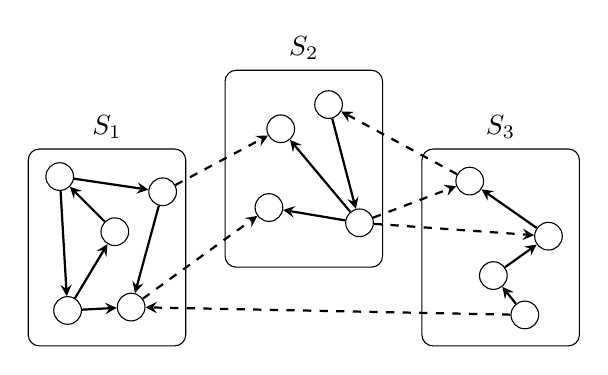
\begin{tikzpicture}[node distance=1cm]

    \node (s1) [server,label=$S_1$] {};
    \node (s2) [server, right of=s1,xshift=1.5cm,yshift=1cm,label=$S_2$] {};
    \node (s3) [server, right of=s1,xshift=4cm,label=$S_3$] {};

    \node (v1) [vertex,xshift=-0.5cm,yshift=-0.8cm] {};
    \node (v2) [vertex, above of=v1,xshift=-0.1cm,yshift=0.7cm] {};
    \node (v3) [vertex, above of=v1,xshift=0.6cm] {};
    \node (v4) [vertex, below right of=v3,xshift=-0.5cm,yshift=-0.25cm] {};
    \node (v5) [vertex, above right of=v3,xshift=-0.1cm,yshift=-0.2cm] {};
    \node (v6) [vertex, right of=v5,xshift=0.5cm,yshift=0.8cm] {};
    \node (v7) [vertex, below of=v6, xshift=-0.15cm,yshift=0cm] {};
    \node (v8) [vertex, right of=v4, yshift=-0.1cm,xshift=4cm] {};
    \node (v9) [vertex, above of=v8,xshift=-0.4cm,yshift=-0.5cm] {};
    \node (v10) [vertex, above of=v9,xshift=-1.7cm,yshift=-0.33cm] {};
    \node (v11) [vertex, right of=v9,yshift=0.5cm,xshift=-0.3cm] {};
    \node (v12) [vertex, above of=v11,yshift=-0.3cm,xshift=-1cm] {};
    \node (v13) [vertex, above right of=v6,yshift=-0.4cm,xshift=-0.1cm] {};
    \draw [local] (v2) -- (v1);
    \draw [local] (v1) -- (v3);
    \draw [local] (v3) -- (v2);
    \draw [local] (v2) -- (v5);
    \draw [local] (v1) -- (v4);
    \draw [local] (v5) -- (v4);
    \draw [dist] (v5) -- (v6);
    \draw [dist] (v4) -- (v7);
    \draw [dist] (v8) -- (v4);
    \draw [local] (v8) -- (v9);
    \draw [local] (v9) -- (v11);
    \draw [local] (v10) -- (v7);
    \draw [dist] (v10) -- (v12);
    \draw [dist] (v12) -- (v13);
    \draw [local] (v10) -- (v6);
    \draw [dist] (v10) -- (v11);
    \draw [local] (v13) -- (v10);
    \draw [local] (v11) -- (v12);
    \end{tikzpicture}
  \caption{Local and distributed edges}
  \Description{Graph representation.}
  \label{dist-graph}
\end{figure}


Adjacency lists can now contain edge pointers to vertices on remote servers. Maintaining reciprocal consistency for distributed edges is challenging - especially given an architecture employed by contemporary distributed graph databases (\cite{janusgraph}, \cite{TitanDB}). Often an existing BASE database is used for storage, which is then adapted with a query language expressed in terms of edges and vertices along with some gluecode to bind that interface to the underlying database - we refer to such systems as BASE distributed graph databases\footnote{Typically, each partition is replicated for fault tolerance and availability, these issues are beyond the scope of this paper.}. Superficially, opting for this design appears to be a good choice: the application programmer has the modeling convenience of graphs with the operational characteristics from the underlying BASE database.

However, the problem with this design is the (lack of) transactional semantics is inherited from the underlying database. BASE databases seldom provide guarantees for multi-operation, multi-object transactions that span partitions. This lack of concurrency control across partitions makes it possible for concurrent updates to interleave in a manner that violates reciprocal consistency of distributed edges\footnote{When operating without concurrency control it is equally possible that local edges become reciprocal consistent, however primitives provided by BASE databases are typically sufficient to ensure reciprocal consistency for local edges.}. Earlier work investigated how the lack of concurrency control across partitions can undermine reciprocal consistency of distributed edges, causing irreversible corruption that spreads at alarmingly rates (\cite{Ezhilchelvan2018}, \cite{Webber2019}). This process is explained in Section \ref{sec:db-corruption}.

\begin{figure*}[ht]
  \centering
  \begin{subfigure}[b]{0.3\textwidth}
    \centering
    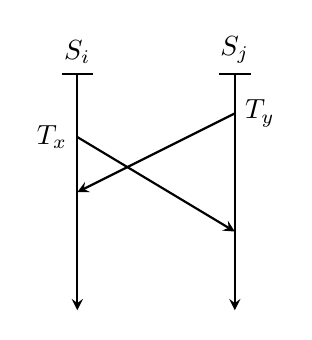
\begin{tikzpicture}
      \draw [thick] (1.3,3) -- (1.7,3);
      \draw [thick,<-,>=stealth] (1.5,0) -- (1.5,3) node[anchor=south] {$S_i$};
      \draw [thick] (3.3,3) -- (3.7,3);
      \draw [thick,<-,>=stealth] (3.5,0) -- (3.5,3) node[anchor=south] {$S_j$};
      \draw [thick,<-,>=stealth] (1.5,1.5) -- (3.5,2.5)  node[right] {$T_y$};
      \draw [thick,->,>=stealth] (1.5,2.2) node[left] {$T_x$} -- (3.5,1);
    \end{tikzpicture}
    \caption{}
    \label{fig:tx-ty}
  \end{subfigure}%
  \begin{subfigure}[b]{0.3\textwidth}
    \centering
    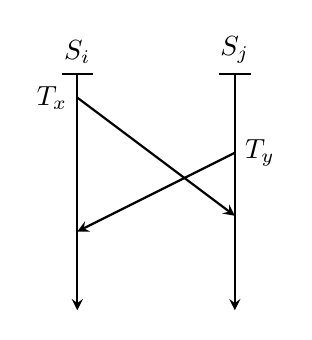
\begin{tikzpicture}
      \draw [thick] (5.3,3) -- (5.7,3);
      \draw [thick,<-,>=stealth] (5.5,0) -- (5.5,3) node[anchor=south] {$S_i$};
      \draw [thick] (7.3,3) -- (7.7,3);
      \draw [thick,<-,>=stealth] (7.5,0) -- (7.5,3) node[anchor=south] {$S_j$};
      \draw [thick,<-,>=stealth] (5.5,1) -- (7.5,2)  node[right] {$T_y$};
      \draw [thick,->,>=stealth] (5.5,2.7) node[left] {$T_x$} -- (7.5,1.2);
    \end{tikzpicture}
    \caption{}
\label{fig:ty-tx}
  \end{subfigure}%
  \begin{subfigure}[b]{0.3\textwidth}
    \centering
    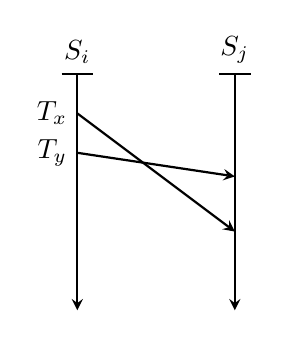
\begin{tikzpicture}
      \draw [thick] (9.3,3) -- (9.7,3);
      \draw [thick,<-,>=stealth] (9.5,0) -- (9.5,3) node[anchor=south] {$S_i$};
      \draw [thick] (11.3,3) -- (11.7,3);
      \draw [thick,<-,>=stealth] (11.5,0) -- (11.5,3) node[anchor=south] {$S_j$};
      \draw [thick,->,>=stealth] (9.5,2.5)  node[left] {$T_x$} -- (11.5,1) ;
      \draw [thick,->,>=stealth] (9.5,2) node[left] {$T_y$} -- (11.5,1.7);
    \end{tikzpicture}
    \caption{}
    \label{fig:same-side}
  \end{subfigure}%
  \caption{Possible interleavings of concurrent transaction's writes to a distributed edge spanning servers $S_i$ and $S_j$ by transactions $T_x$ and $T_y$. In \subref{fig:tx-ty} $T_y$ begins writing to the distributed edge before $T_x$, in \subref{fig:ty-tx} the converse is true, else they are equivalent. In \subref{fig:same-side} both transactions begin writing at the same server but overlap in the network and arrive out-of-order.}
  \label{conf-scen}
\end{figure*}


\section{Reciprocally Inconsistent Distributed Edges}
\label{sec:db-corruption}

Suppose that the edge \texttt{(a)-[:\textcolor{green}{WROTE}]->(b)} is a distributed edge, with vertices \emph{a} and \emph{b} in servers $S_i$ and $S_j , j\neq i$,  respectively.
When a transaction writes this edge $ab$,
\begin{enumerate}
\item two writes are performed: reciprocal entries in the adjacency lists of both \emph{a} and \emph{b} are updated, and
\item write order is unconstrained: a transaction is equally likely to write \emph{a} then \emph{b} as it is to write \emph{b} then \emph{a}.
\end{enumerate}

Concurrent transactions $T_x$ and $T_y$ can interleave in the following three ways and each one is depicted in Fig \ref{fig:conf}:
\begin{enumerate}[(a)]
\item $T_x$ starts before $T_y$; it writes $a$ at $S_i$ first and then proceeds to $S_j$ across the network; $T_y$ operates the other way round, beginning with $S_j$ and proceeding to $S_i$ (see Fig \ref{fig:a}). The net effect is:  $T_x \rightarrow T_y$ at $S_i$ and at  $T_y \rightarrow T_x$ at $S_j$, where  $T \rightarrow T'$ at $S$ denotes that $T$ \emph{precedes} $T'$ at server $S$.
\item Same as the previous case, except that $T_y$ starts earlier than $T_x$ (see Fig \ref{fig:b}).
\item Same net effect as in previous two cases, except that both $T_x$ and $T_y$ start their first writes at $S_i$, $T_x \rightarrow T_y$, but $T_y$ overtakes $T_x$ in reaching $S_j$ where $T_y \rightarrow T_x$ (see Fig \ref{fig:c}).
\end{enumerate}

We could envisage three more corresponding cases (a') - (c') where the roles of $T_x$ and $T_y$ in cases (a) - (c) are simply interchanged; e.g., in case (a'), $T_y$ starts before $T_x$, writes $a$ at $S_i$ first and then proceeds to $S_j$ across the network; $T_x$ operates the other way round, beginning with $S_j$ and proceeding to $S_i$. Thus, there are only 6 ways concurrent $T_x$ and $T_y$ can interleave. The arguments we make based on cases (a) - (c) of Fig \ref{fig:conf} equally apply, by symmetry, to cases (a') - (c') and so, for brevity, we will not consider the latter.

At the end of each case in Fig \ref{fig:conf}, the last update on $a$ is by $T_y$ and that on $b$ is by $T_x$. Unless updates of $T_x$ and $T_y$ are commutative, $ab$ cannot be reciprocally consistent. As an example, suppose that $T_x$ deletes the \emph{wrote} edge while $T_y$ concurrently appends a property \emph{year}:
\begin{Verbatim}[commandchars=\\\{\},fontsize=\small,xleftmargin=.2in]
\textcolor{grey}{// Tx}
\textcolor{blue}{MATCH} (a:\textcolor{green}{Person})-[w:\textcolor{green}{WROTE}]->(b:\textcolor{green}{Book})
\textcolor{blue}{WHERE} a.\textcolor{red}{name} = 'Tolkien' \textcolor{blue}{AND} b.\textcolor{red}{title} = 'The Hobbit'
\textcolor{blue}{DELETE} w

\textcolor{grey}{// Ty}
\textcolor{blue}{MATCH} (a:\textcolor{green}{Person})-[w:\textcolor{green}{WROTE}]->(b:\textcolor{green}{Book})
\textcolor{blue}{WHERE} a.\textcolor{red}{name} = 'Tolkien' \textcolor{blue}{AND} b.\textcolor{red}{title} = 'The Hobbit'
\textcolor{blue}{SET} w.\textcolor{red}{year} = 1937
\end{Verbatim}
\begin{figure}[htp]
  \centering
  \begin{subfigure}{\linewidth}
    \centering
    \begin{tikzpicture}[node distance=2cm]
  \node (v1) [big_vertex,xshift=0cm,yshift=0cm] {\small{\texttt{a:\textcolor{green}{Person}}}};

  \node (v2) [big_vertex,xshift=5cm,yshift=0cm] {\small{\texttt{b:\textcolor{green}{Book}}}};

  \node [below of=v1,yshift=1cm] {\small{\texttt{\textcolor{red}{name}:Tolkien}}};
  \node [below of=v2,yshift=1cm] {\small{\texttt{\textcolor{red}{title}:The Hobbit}}};

  \draw [thick,->,>=stealth] (0.8,0)  -- node [midway,above] {:\textcolor{green}{\small{\texttt{WROTE}}}} node [midway,below] {\small{\texttt{\textcolor{red}{year} = 1937}}} (2.4,0);
\end{tikzpicture}

    \caption{Logical view.}
    \label{hc-edge}
  \end{subfigure}
  %
  \begin{subfigure}{\linewidth}
    \vspace{2ex}
    \centering
        \begin{tikzpicture}[node distance=2cm,scale=0.6,every node/.style={transform shape}]

      \record(
      0,
      \small{\texttt{a:Person}},
      \small{\texttt{name:Tolkien}},
      $\boldsymbol{\rightarrow}$ \textbf{\small{\texttt{wrote b}}},
      \texttt{edge},
      \texttt{edge}
      );

      \record(
      -1,
      \small{\texttt{b:Book}},
      \texttt{property},
      \small{\texttt{title:The \hspace{-0.15cm} Hobbit}},
      ,
      \texttt{edge}
      );

      \record(-2,
      \small{\texttt{vertex id}},
      \texttt{property},
      \texttt{property},
      \texttt{edge},
      \texttt{edge}
      );


      \spaceRecord(-3)

      \record(-4,
      \small{\texttt{vertex id}},
      \texttt{property},
      \texttt{edge},
      \texttt{edge},
      \texttt{edge}
      );

    \end{tikzpicture}

    \caption{Storage view.}
    \label{hc-db-rep}
  \end{subfigure}%
  \caption{Logical and storage views of a reciprocally inconsistent edge \emph{ab}.}
  \label{hc}
\end{figure}
The interleaving patterns depicted in Fig \ref{fig:conf} leave $ab$ reciprocally inconsistent, as shown in Fig \ref{hc}.

When $T_x$ and $T_y$ do not interleave,  either $T_y \rightarrow T_x$ or $T_x \rightarrow T_y$ holds at both servers $S_i$ and $S_j$; in that case, the last update on \emph{both} $a$ and $b$ would be by either $T_x$ or $T_y$, respectively. That is, when transactions update at both ends of $ab$  in \emph{some} arbitrarily chosen but identical order, $ab$ is left  reciprocally consistent after each transaction's update.

When interleaving updates leave $ab$ reciprocally inconsistent, $ab$ can be said to have become \emph{half-corrupted} because if $T_y \rightarrow T_x$ is the chosen order between $T_y$ and $T_x$, then the edge pointer in $b$ of $ab$ is in error; otherwise, the edge pointer in $a$ is erroneous. Thus, a reciprocally inconsistent edge $ab$ certainly has a corrupt half but the question of which half is corrupt has been left open.

Suppose that a future transaction $T_w$ \emph{first} reads the edge pointer of reciprocally in consistent $ab$, say, at vertex $a$. (Note that when $T_w$ reads any edge, it does not check for reciprocally consistency). At that moment, $T_w$ (implicitly) chooses the order $T_x \rightarrow T_y$ and thereby invalidates the other order $T_y \rightarrow T_x$ that prevails at vertex $b$. Thus, from that moment onward, the $b$ end of edge $ab$ becomes the corrupt end.

If no transaction ever reads the edge pointer at vertex $b$, then the order $T_x \rightarrow T_y$ effectively prevails and the half-corruption of $ab$ remains invisible to the rest of the database. However, if $T_z$ is to subsequently read the edge pointer at $b$ and write another edge based on what it read, i.e., The Hobbit has unknown author, then it is introducing updates not consistent with what $T_w$ read earlier; it thus introduces \emph{semantic corruption} into the database. Further writes based on reading semantically corrupt data also spread corruption.

A database is said to be \emph{operationally corrupt} when a significant proportion of its data records are in a semantically corrupt state. As stated earlier, we had shown that 10\%  of a distributed graph database can become semantically corrupt well within the system lifetime itself (\cite{Ezhilchelvan2018}, \cite{Webber2019}).

Two more relevant remarks on past works:
a half-corrupted edge is due to a \emph{dirty write} (ANSI \emph{P0} \cite{Berenson1995}, Adya \emph{G0} \cite{Adya2000}) in the context of distributed graph databases. If the database provides the ANSI isolation level \emph{Read Uncommitted}, it will identically order the writes of concurrent transactions and this would prevent all interleaving patterns shown in Fig \ref{fig:conf} and thus avert half-corruption altogether.


\section{\tDelta Protocol}
\label{sec:tdelta-protocol}

A straightforward solution to preventing dirty writes is for transactions to take long duration write locks \cite{Berenson1995}, releasing them only once the acquiring transaction has committed or aborted. To prevent deadlock a policy such as \texttt{NO_WAIT} deadlock detection is used, which was shown to be the optimal policy in a distributed, partitioned database \cite{Harding2017}.

Our \tDelta protocol employs principles behind all these well-tested strategies but has two crucial differences:
\begin{itemize}
\item No locks are used.
\item A write operation need not await until the preceding write commits but can proceed if at least $\Delta$ duration (measured in local clock) has elapsed.
\end{itemize}

These differences lead to several advantages in the context of graph databases. Firstly, a subset of edges are traversed and modified with a high frequency e.g. critical sections of motorway in a road network, leading to high contention. Secondly, graph transactions tend to be longer-lived than transactions in relational databases. Waiting for earlier writes on edges by long running transactions to commit, these frequently accessed edges significantly limit concurrency and reduce throughput. With these concerns in mind we developed the \tDelta protocol, which aimed at preventing edges becoming half-corrupted and hence quashing the seed of corruption whilst keeping performance at an acceptable level.\footnote{The \tDelta protocol is solely a concurrency control mechanism for distributed edges, guarantees about vertices, local edges are beyond the scope of this paper.}

\subsection{Protocol Description}
\label{sec:protocol-description}

The \tDelta Protocol has five rules:
\begin{enumerate}
\item A transaction's write on an end pointer of an edge is initially tentative which would become permanent only if that transaction is permitted to commit.
\item A tentative write is possible if the end pointer is either in a permanent state or the immediately preceding tentative write was done at least $\Delta$ time before (where time is measured as per local clock).
\item If a transaction successfully performs all its tentative writes, then it is permitted to commit; otherwise, it must abort.
\item A transaction commits, when all its tentative writes are made permanent, e.g., using an atomic commitment protocol.
\item Tentative writes of an aborting transactions are ignored. An ignored tentative write can make a new transaction abort for up to $\Delta$ time after it was created; it is harmless thereafter and can be garbage collected at any time.
\end{enumerate}

\subsection{Correctness Reasoning}
\label{sec:corr-reas}

Let us define $\delta$ as the bound estimate on the interval that may elapse between a transaction writing one end of a distributed edge at one server and writing the other end of the same edge at another server.

Let $\Delta$ be chosen such that $\Delta > \delta$.
Now consider the interleaving in Figure \ref{fig:b} and let $t_x$ be the (global) time when $T_x$ starts at server $S_i$; similarly $t_y$ be the time $T_y$ starts at server $S_j$.
Note $t_y < t_x$, i.e. $(t_x - t_y) > 0$.

Say, $T_y$ reaches $S_i$ at time $t_y + d$, where $d$ is the actual time elapsed between completing a tentative write at one end and starting at another end, let us assume that $d \leq \delta$.
When $T_y$ arrives at $S_i$ it will find a tentative write done at time $t_x$.
In this case, $t_y + d - t_x = d - (t_x-t_y) < d \leq \delta < \Delta$; so, $T_y$ will abort, preventing writes from interleaving and half-corrupting the edge.
A similar arguments can be made for the scenario in with Figure \ref{fig:b}, where $t_y > t_x$ and $T_x$ will abort because it will find out, on reaching server $S_j$ for the final tentative write, that $t_x +d - t_y = d - (t_y-t_x) < d <= \delta < \Delta$.
For the interleaving in Figure \ref{fig:same-side}, if $t_y - t_x > \Delta$, then $T_y$ cannot overtake $T_x$ at $S_j$.

Assume that $d > \delta$, i.e., the estimate $\delta$ does not hold at this moment.
In Figure \ref{fig:b} interfering writes are avoided only if $t_y + d - t_x = d - (t_x-t_y) < d < \Delta$ otherwise, reciprocal inconsistency occurs.
In Figure \ref{fig:a} interfering writes are avoided only if $t_x + d - t_y = d - (t_y-t_x) < d < \Delta$ otherwise, reciprocal inconsistency occurs.
Thus, in the extreme case $t_x = t_y$ and reciprocal consistency is not guaranteed if $\Delta < d$ when the latter exceeds its upper bound estimate $\delta$.
For Figure \ref{fig:c}, interfering writes are avoided only if $(t_y + d) - (t_x + d) = (t_y- t_x) < d < \Delta$ other reciprocal inconsistency occurs.

% This protocol is strictly weaker than Read Uncommitted isolation, ensuring only writes to distributed edge are totally ordered, preserving reciprocal consistency. The benefit of this approach is reduced contention on frequently accessed distributed edges, as the time a transaction has exclusive access to a given distributed edge is decreased.

% In summary, the \tDelta protocol attempts to prevent the occurrence of half-corrupted distributed edges by aborting transactions but if $\Delta$ is exceeded edge can become half-corrupted and process of corruption described in Section \ref{sec:db-corruption} can still occur. Two questions naturally arise regards the performance of the protocol. For different values of $\Delta$:
% \begin{itemize}
% \item Given distributed edges can still become half-corrupted if $\Delta$ is exceeded, by how much time does the protocol increase the time until operational corruption?
% \item How many transactions are aborted as a result of the protocol?
% \end{itemize}


In summary, the \tDelta protocol eliminates interleaving of transactions during edge writes, so long as $\Delta$ remains larger than the interval $d$ that elapses between a transaction completing its write at one end of a distributed edge and starting at the other end.
Since the exact value of $d$ taken by a transaction cannot be precisely known in advance, its bound $\delta$ is estimated with the best effort and we choose $\Delta > \delta$.

The larger the value of $\Delta$ used, the more likely is that $\Delta > d$ holds and half-corruption and thereby operational corruption are averted; also, the more likely is that one or more of concurrent transactions will find their tentative write within $\Delta$ time of each other and choose to abort.
Our performance evaluation of the protocol will therefore involve measuring the folowing two metrics for various values of $\Delta$:
\begin{itemize}
\item Time taken for 10\% of a large database to be corrupted due to the introduction of half-corruption, and
\item Number of transactions being aborted per second.
\end{itemize}
e let $d$ be an exponentially distributed random variable with mean $\mu$, $D\sim \exp(\mu)$. Therefore, the probability of $d$ exceeding $\Delta$ is given by $P(D > \Delta) = e^{(-\mu \Delta)}$.

%The two paragraphs (The protocol leverages... edge is lost) can be commented out.

%Figures 5 and 6 can be removed.

% The protocol leverages the fact that a transaction that writes at one end of a distributed edge, must then immediately write the other end. It is then assumed that the network delay between two servers can be predicted to be some $\Delta$. All writes are temporary and assumed to be made permanent by a later atomic commitment protocol once the transaction has completed. From this, a distributed edge write is allowed to proceed provided there is no other temporary write preceding it within $\Delta$; measured as per the local clock time. Figure \ref{delta-abort} shows an instance of the protocol preventing the interleaving in Figure \ref{conf-scen} (c), $T_x$ overtakes $T_y$ but is aborted when arriving at $S_j$ as $T_y$ has already wrote tentatively within $\Delta$. An aborted transaction, aborts any and every previous tentative write that it may have successfully completed. This protocol avoids all conflict scenarios in Figure \ref{conf-scen} provided $\Delta$ is not exceeded.



% \begin{figure}[H]
%   \centering
%   \begin{tikzpicture}[node distance=2cm]
%     % s1
%     \draw [thick] (1.3,3) -- (1.7,3);
%     \draw [thick,<-,>=stealth] (1.5,0) -- (1.5,3) node[anchor=south] {$S_i$};
%     % s2
%     \draw [thick] (3.3,3) -- (3.7,3);
%     \draw [thick,<-,>=stealth] (3.5,0) -- (3.5,3) node[anchor=south] {$S_j$};

%     \draw [thick,->,>=stealth] (1.5,2.5) node[left] {$T_x$} -- (3.5,0.5);
%     \draw [thick,->,>=stealth] (1.5,2) node[left] {$T_y$} -- (3.5,1.8);

%     \draw [thick,<->,>=stealth] (3.7,0.5) -- (3.7,1.8) node[midway,right] {$< \Delta$};

%   \end{tikzpicture}
%   \caption{An example of the \tDelta protocol preserving reciprocal consistency.}
%   \label{delta-abort}
% \end{figure}

% Correctly choosing $\Delta$ is paramount, as if it is exceeded all three conflict scenarios can still occur, resulting in half-corrupted edges and the spread of semantic corruption. Figure \ref{corruption-again} displays an example when the \tDelta protocol fails to maintain reciprocal consistency. The network delay between $S_i$ and $S_j$ is sufficiently large the total ordering of writes to the distributed edge is lost.

% \begin{figure}[H]
%   \centering
%   \begin{tikzpicture}[node distance=2cm]
%     \draw [thick] (1.3,3) -- (1.7,3);
%     \draw [thick,<-,>=stealth] (1.5,0) -- (1.5,3) node[anchor=south] {$S_i$};
%     \draw [thick] (3.3,3) -- (3.7,3);
%     \draw [thick,<-,>=stealth] (3.5,0) -- (3.5,3) node[anchor=south] {$S_j$};
%         \draw [thick,->,>=stealth] (1.5,2.7) node[left] {$T_x$} -- (3.5,0.8);
%     \draw [thick,<-,>=stealth] (1.5,1) -- (3.5,2.2)  node[right] {$T_y$};

%     \draw [thick,<->,>=stealth] (4.2,1) -- (4.2,2.2) node[midway,left] {$> \Delta$};
%     \draw [thick,<->,>=stealth] (0.8,1) -- (0.8,2.5) node[midway,right] {$> \Delta$};
%   \end{tikzpicture}
%   \caption{An example of the \tDelta protocol failing to preserve reciprocal consistency.}
%   \label{corruption-again}
% \end{figure}


\section{Performance Evaluation Strategies}
\label{sec:modeling}

To assess the time to operational corruption, we reused the model that we developed in \cite{Ezhilchelvan2018} and adapted it for the \tDelta protocol.
For completeness, the model is briefly explained first before we discuss the adaptation.
We note that an empirical evaluation of the time to operational corruption using a real system would be impractical due to the sheer length of time and the cost it would take to run the experiment.
(For certain values of $\Delta$, the model predicts anywhere between 1-75 years for operational corruption! Details are to follow.)

The model of \cite{Ezhilchelvan2018} assumes that transactions arrive in a Poisson stream with rate $\lambda$ transactions per second (TPS, for short).
Each transaction performs a random number ($K$) of read operations and then updates a single edge.

To model a scale-free graph, edges in the distributed database are divided into $T$ types, $i = 1, 2, \ldots, T$.
Type-1 edges represent the most popular edges to be accessed by transactions and type-$T$ edges are the least popular. Popular edges are smaller in number compared to the less popular ones.
$N$ denotes the total number of edges in the database.
For all edge types, a fraction $f$ are distributed.

At time $0$, all edges are assumed to be clean (free from corruption); thereafter, an edge can be in one of four states:
\begin{enumerate}
\item Local and clean.
\item Distributed and clean.
\item Distributed and half-corrupted.
\item Local or distributed and semantically corrupted.
\end{enumerate}

The delay $d$ is the time interval that elapses between a transaction completing its tentative write at one end of a distributed edge and starting at another end. It constitutes the window for concurrent transactions to interleave as portrayed in Fig \ref{fig:conf}. It is assumed to be exponentially distributed with mean $ 1/ \mu$ (i.e., at rate $\mu$).

The model parameters now enable us to compute the probability $q_i$ that a transaction updating a clean type-$i$ distributed edge, leaves it half-corrupted, in the absence of any concurrency control mechanism. (Our earlier work in \cite{Ezhilchelvan2018} assumes no concurrency control). These probabilities, $q_i, 1 \leq i \leq T$, are then used to compute transition rates $a_{j,k}$ between state $j$ to $k$, $1 \leq j,k \leq 4$. (Since local and distributed edges are fixed, $a_{1,2} = a_{2,1} = 0$.)

The rates $a_{j,k}$ are in turn used to simulate the spread of corruption within the database to estimate the first passage time $U_{\gamma}$  for a fraction ${\gamma}$ of $N$ edges to enter the state 4. (When $\gamma N$ edges become semantically corrupt, the database becomes operationally corrupt.)  The reader is directed to \cite{Ezhilchelvan2018} and \cite{Webber2019} for a granular discussion of the initial model.

\paragraph{\tDelta Protocol Adaptation}
Our concurrency protocol reduces the probabilities $q_i, 1 \leq i \leq T$ and we compute $q^{new}_i$ as shown in Appendix \ref{sec:deriv-confl-prob}.
The new probabilities $q^{new}_i$ are used in the model and simulations of \cite{Ezhilchelvan2018} to estimate $U_{\gamma}$.

\paragraph{Number of aborts per second.} To evaluate this metric for various values of $\Delta$, a second simulation that focuses specifically on the subset of most frequently accessed distributed edges was performed.

Note that both metrics that we set out to evaluate will be influenced by several parameters that characterize the database and other aspects:
\begin{itemize}
\item \emph{Database Size}. Size is expressed by the total number of edges $N$, and the fraction $f$ of distributed edges.
\item \emph{Workload}. Measured as transactions per second (TPS). Significant for measuring $U_{\gamma}$ are: the fraction of this load that writes after reads and the number of reads that precede a write.
\item \emph{Distributed Write Delays and Choosing $\Delta$}. The smaller the delays the less likely the bound $\Delta$ is violated. Conversely, smaller $\Delta$ is the more likely the bound $\Delta$ is violated.
\end{itemize}


\section{Evaluation}
\label{sec:evaluation}

The graph analyzed consisted of seven edge types, $N_1=10^4, N_2=10^5, N_3=10^6, N_4=10^7,  N_5=10^8, N_6=10^9, N_7=10^{10}$, totaling 11 billion edges, with access probabilities $p_1 =0.5, p_2 =0.25, p_3=0.13, p_4=0.06, p_5=0.03, p_6=0.02$ and $p_7 =0.01$; a graph of this size would have approximately 1 billion vertices.
The number of read operations per query is geometrically distributed starting at $2$, with an average of $15$, before a write.
In all edge types, a fraction $0.3$ are distributed, the remainder are local; in proportion with a good graph partitioning algorithm.
The delay $d$ between a transaction completing a tentative write at one end and starting at another end is exponential distributed with a mean of $5ms$.
The database is initial clean and considered to be corrupted when $10$\% ($\gamma = 0.1$) of all edges are corrupted.
The time taken until operational corruption $U$, is measured in days.
$U$ considered for a range of transaction arrival rates, $\lambda = (1000, ..., 10000)$; a typical graph workload comprises of 90\% read-only transactions and 10\% read-write transactions \cite{Angles2020}, hence the chosen range reflects a total workload of $\lambda = (10000, ..., 100000)$.
The following $\Delta$ values were considered $\Delta = 50, 75, 100ms$.
For each $\Delta$ the probability that $d$ exceeds $\Delta$ is $P(D > \Delta) = 4.5 \time 10^{-5}, 3.1 \times 10^{-7}, 2.1 \times 10^{-9}$ respectively.

The results for measuring the impact of $\Delta$ on the time until operational corruption are given in Figure \ref{time-to-corruption-results}.
Under no isolation, $U$ ranges between 50-500 days.
For $50ms$ this increases to 1-75 years. For $\Delta = 75, 100ms$ the time to corruption vastly exceeds lifetime of any system making data corruption resulting from half-corrupted edges of little practical concern.

\begin{figure}[h]
  \centering
  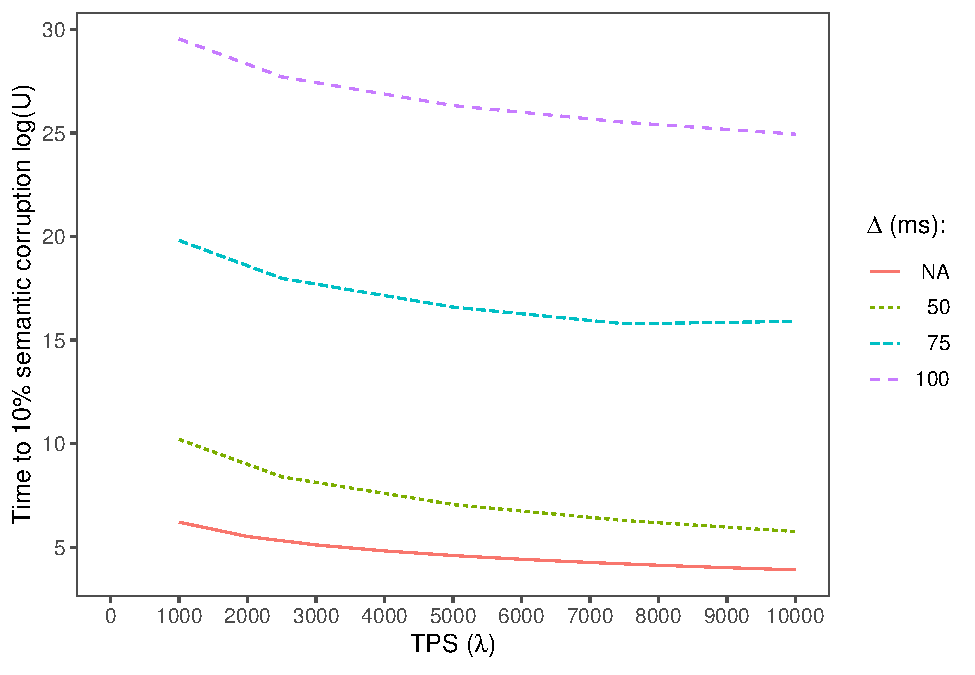
\includegraphics[width=\linewidth]{./figures/delta}
  \caption{Time until operational corruption.}
  \label{time-to-corruption-results}
\end{figure}

The number of aborts per second for $\Delta = 50, 75, 100ms$ are given in Figure \ref{aborts-results} for the most popular edge type, $N=10^4$. The simulation was ran for 10 seconds for a range of transaction arrival rates, $\lambda = (1000, ..., 10000)$. For $\Delta = 50$ the abort rate varies between $1-5\%$, this increases to between $1-7\%$ and $1-9\%$ for $\Delta = 75$ and $\Delta = 100$ respectively.

\begin{figure}[h]
  \centering
  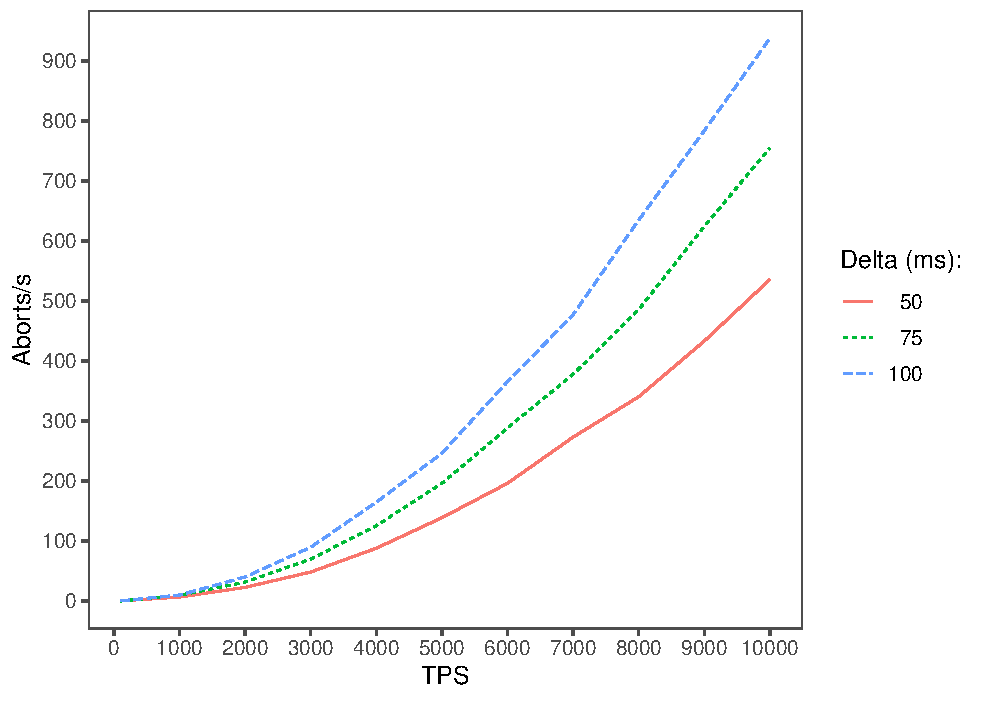
\includegraphics[width=\linewidth]{./figures/aborts}
  \caption{Number of aborts per second.}
  \label{aborts-results}
\end{figure}


\section{Conclusions}

Database concurrency control has been a long researched area, however to the best of our knowledge this is first attempt at a developing protocol specific for distributed graph databases. We presented a lightweight protocol for providing reciprocal consistency and mitigating the problem of high contention in a distributed graph database. The \tDelta protocol leverages the fact writes to distributed edges always consists of two sequential writes to entries in the adjacency lists of vertices the edge connects. The protocol provides guarantees weaker than Read Uncommitted isolation (the weakest ANSI isolation level). However, such a mechanism is believed to be valuable in practice, given the popularity of BASE distributed graph databases and the rate at which corruption can spread if left unchecked. Simulations indicate the protocol rules out corruption resulting from half-corrupted distributed edges in realistic database lifetime, with the abort rate being in a reasonable range. For future work, we intend on implementing the protocol to assess the validity of the simulations and measure performance against a BASE distributed graph database operating without any concurrency control. Moreover, we plan on investigating the suitability of higher isolation levels in a distributed graph database, \textbf{Read Atomic} isolation \cite{Bailis2014} seems particularly well suited.



\bibliographystyle{ACM-Reference-Format}
\bibliography{papoc}

\appendix

\section{Derivation of Conflict Probability}
\label{sec:deriv-confl-prob}

Under the \tDelta protocol each interleaving in Figure \ref{fig:conf} can be given a probability of occurring. Figures \ref{fig:a} and \ref{fig:b} are equivalent and can be summarized by the same probability. Letting $t_x = 0$, the probability that $T_x$ and $T_y$ conflict can be formulated as: $$ P \left[ ( T_x >  \Delta + D) \cap (T_y > \Delta-D) \right]$$ The arrival times of $T_x,T_y$ are assumed exponentially distributed, $T \sim \exp (\rho)$.
Where, $ \rho  = \frac{\lambda P_i}{2N_i}$, the probability a given operation accesses the incorrect record of a half-corrupted edge of type $i$.
The probability of $d$ exceeding $\Delta$ is exponentially distributed with mean $\mu$, $D\sim \exp(\mu)$.
Therefore,
\begin{dmath*}
   q^{new}_{i} =  {P \left[ ( T_1 >  \Delta + D) \cap (T_2 > \Delta-D)  \right]} \\
   =  \int_{0}^{\Delta}  \frac{\lambda P_i}{2 N_i} e^{-\frac{\lambda P_i}{2 N_i} d} e^{-\mu (\Delta+d)} e^{-\mu (\Delta-d)} dd + \int_{\Delta}^{\infty} \frac{\lambda P_i}{2 N_i} e^{-\frac{\lambda P_i}{2 N_i} d} e^{-\mu (\Delta+d)} dd  \\
   =  e^{-2 d \mu} - \left( \frac{\mu}{\frac{\lambda P_i}{2 N_i} + \mu} \right) e^{-(\frac{\lambda P_i}{2 N_i}+ 2\mu)d} \\
 \end{dmath*}
To simply the derivation of the conflict probability we assume FIFO which rules out the interleaving in Figure \ref{fig:c}.
 % To choose to bound $\Delta$ consider the probability of the message delay exceeding  $\Delta$.
 % \begin{align*}
 %   P \left[ M > \Delta \right] & = 1 - e^{- \delta \Delta} \\
 %   1 - e^{- \delta \Delta} & = 1 - \epsilon \\
 %   e^{- \delta d} & = \epsilon  \\
 %   \Delta & = - \frac{\ln(\epsilon)}{\delta}
 % \end{align*}

%  Substituting $\Delta$ into the above equation yields the conflict probability for a given $\epsilon$. For example, $ e = 0.001$ gives a $0.001$ \% probability the message delay exceeds $\Delta$, for this  $\Delta = 0.035s$
% \begin{align}
%   e^{- \lambda d} =  e^{-\delta d \frac{\lambda}{\delta}} = \epsilon^{\frac{\lambda}{\delta}} \label{eqn7}
% \end{align}
% Therefore, from (\ref{eqn5} and  (\ref{eqn7}),
% \begin{align}
%   & = \epsilon^2 - \frac{\delta}{\frac{\lambda P_i}{2 N_i} + \delta} e^{-\frac{\lambda P_i}{2 N_i} d} \epsilon^2 \\
%   & = \epsilon^2 \left[1 -\frac{\delta}{\frac{\lambda P_i}{2 N_i} + \delta} e^{-\frac{\lambda P_i}{2 N_i} d} \right]
% \end{align}


% Where, $ E \left[ T_1 \right] = E \left[ T_2\right] = \frac{1}{\delta}$.
% Therefore, $$ f(x) =\frac{\lambda P_i}{2N_i} e^{-\frac{\lambda P_i}{2N_i} x} $$

%  % =   \int_{0}^{d}  \frac{\lambda P_i}{2 N_i} e^{-\frac{\lambda P_i}{2 N_i} x} e^{-\delta 2 d} dx +  \int_{d}^{\infty} \frac{\lambda P_i}{2 N_i} e^{-\delta d} e^{-(\frac{\lambda P_i}{2 N_i} + \delta)x}  dx  \\
%  %        =   e^{-2 d \delta} \left[1 - e^{-\frac{\lambda P_i}{2 N_i} d} \right] + \frac{\frac{\lambda P_i}{2 N_i} e^{-\delta d}}{\frac{\lambda P_i}{2 N_i} + \delta} e^{-(\frac{\lambda P_i}{2 N_i} + \delta)d} \\


\end{document}
\endinput
